% Implementation Details...

\section{Implementation Details for Branching}
\label{sec:facerefinement}

We will now make a detailed examination of the internal structure
of exceptional regions.

A {\it refinement\/} $\tildeF$ of a face $F$ of a plane graph $G$
is a set $\tildeF$ of faces  such that
    \begin{enumerate}
    \item The intersection of
the vertex set of $G$ with that of $\tildeF$ is the set $F$.
    \item $\tildeF \cup\{F^{op}\}$ is a plane graph.
    \end{enumerate}
We use refinements of faces to describe the internal structure of
faces.

We introduce indexing sets $\marku{FACE-\tildeF }$,
$\marku{VERTEX-\tildeF }$, $\marku{ANGLE-\tildeF }$,
$\marku{EDGE-\tildeF }$, the sets of faces, vertices, angles, and
edges in $\tildeF$, respectively, analogous to those introduced
for $G$.

We create variables
    $\pi[\tildeF]$, and indexed variables
    $$
    \begin{array}{lll}
    \sol\{\marku{FACE-\tildeF }\}, & \sc\{\marku{FACE-\tildeF }\} &
    \tausc\{\marku{FACE-\tildeF }\},\\
    \alpha\{\marku{ANGLE-\tildeF }\}, & y\{\marku{VERTEX-\tildeF }\}, &
    e\{\marku{EDGE-\tildeF }\}.
    \end{array}
    $$
(Variables with names ``$y[v]$'' and ``$e[v,w]$'' were already
created for some $v,w\in \marku{VERTEX-\tildeF }\cap
\marku{VERTEX}$.  In these cases, we use the variables already
created.)

Each vertex $v$ in the refinement will be interpreted either as a
vertex $v^I\in U(D)$, or as the endpoint of an upright diagonal
lying over the standard region $F^I$. We will interpret the faces
of the refinement in terms of the geometry of the decomposition
star $D$ variously as flat quarters, upright quarters, anchored
simplices, and the other constructs of \Part~\ref{part:bounds}.
This interpretation depends on the context, and will be described
in greater detail below.

Once the interpretation of faces is fixed, the interpretations are
as before for the variable names introduced already: $y$, $e$,
$\alpha$, $\sol$.  The lower and upper bounds for $\alpha$ and
$\sol$ are as before.  The lower and upper bounds for $y[v]$ are
$2$ and $2t_0$ if $v^I\in U(D)$, but if $(0,v^I)$ is an upright
diagonal, then the bounds are $[2t_0,2\sqrt2]$. The lower and
upper bounds for $e$ will depend on the context.

\section{Variables related to score}
\label{sec:variable}

The variables $\sc$ are a stand-in for the score $\sigma$ on a
face. We do not call them $\sigma$ because the sum of these
variables will not in general equal the variable $\sigma[F]$, when
$\tildeF$ is a refinement of $F$:
    $$[\sum_{F'\in \tildeF }\sc[F'] \ne \sigma[F]].$$
We will use have a weaker relation:
    $$\sigma[F] \le \sum_{F'\in \tildeF }\sc[F'] + \pi[\tildeF].$$
The variable $\pi[\tildeF]$ is called the penalty associated with
the refinement $\tildeF$.  (Penalties are discussed at length in
\shortversion{\cite{KC}.} \longversion{Sections \ref{sec:penalty}
and \ref{sec:penalty1}.}) The interpretations of $\sc$ and
$\pi[\tildeF]$ are rather involved, and will be discussed on a
case-by-case basis below. The interpretation of $\tausc$ follows
from the identity:
    $$\tausc[F'] = \sol[F']\zeta\pt - \sc[F'],\quad\forall
    F'\in \tildeF .$$

The interpretation of variables that follows might appear to be
hodge-podge at first.  However, they are obtained in a systematic
way. We analyze the proofs and approximations in
Part~\ref{part:bounds}, and define $\sc[F]^I$ as the best
penalty-free scoring approximation that is consistent with the
given face refinement. here are the details.

If the subregion is a flat quarter, the interpretation of $\sc[F]$
is the function $\hat\sigma$, defined in \shortversion{\cite{KC}.}
\longversion{\ref{sec:some-flat}.}  If the subregion is an upright
quarter $Q$, the interpretation of $\sc[F]$ is the function
$\sigma(Q)$ from Section~\ref{sec:scoring}. If the subregion is an
anchored simplex that is not an upright quarter, $\sc[F]$ is
interpreted as the analytic Voronoi function $\vor$ if the simplex
has type $C$ or $C'$, and as $\vor_0$ otherwise. (The types $A$,
$B$, $C$ and $C'$ are defined in Section~\ref{x-2.5}.) Whether or
not the simplex has type $C$, the inequality $\sc[F]\le0$ is
satisfied. In fact, if $\vor_0$ scoring is used, we note that
there are no quoins, and $\phi(1,t_0)<0$.

If the subregion is triangular, if no vertex represents an upright
diagonal, and if the subregion is not a quarter, then $\sc[F]$ is
interpreted as  $\vor$ or $\vor_0$ depending on whether the
simplex has type $A$.  In either case, the inequality
$\sc[F]\le\vor_0$ is satisfied.

In most other cases, the interpretation of $\sc[F]$ is $\vor_0$.
However, if $R$ is a heptagon or octagon, and $F$ has $\ge4$
sides, then $\sc[F]$ is interpreted as $\vor_0$ except on
simplices of type $A$, where it becomes the analytic Voronoi
function.

If $R$ is a pentagon or hexagon, and $F$ is a quadrilateral that is
not adjacent to a flat quarter, and if there are no penalties in the
region, then the interpretation of $\sc[F]$ is the actual score of
the subregion over the subregion. In this case, the score $\sigma_R$
has a well-defined meaning for the quadrilateral, because it is not
possible for an upright quarter in the $Q$-system to straddle the
quadrilateral region and an adjacent region. Consequently, any
erasing that is done can be associated with the subregion without
ambiguity. By the results of \Chaps~\ref{sec:break_piece}
and~\ref{sec:proofs}, we have $\sc[F]\le0$. We also have
$\sc[F]\le\vor_0$.

One other bound that we have not explicitly mentioned is the bound
$\sigma_R(D)< s_n$.  For heptagons and octagons that are not
aggregates, this is a better bound than the one used in the
definition of tameness (Property~\ref{definition:tame:score}). In
heptagons and octagons that are not aggregates, if we have a
subregion with four or more sides, then $\sc[F]< Z(n,k)$ and
$\tausc[F]>D(n,k)$. (See Section~\ref{x-5.5},
Equations~\ref{eqn:tau>D(n,k)} and \ref{eqn:sigma<Z(n,k)}.


The variables are subject to a number of compatibility relations
that are evident from the underlying definitions and geometry.
    $$
    \begin{array}{lll}
    \sol[F'] = \sum_{v\in F'}\alpha[v,F'] - (len[F']-2)\pi,&\forall F'\\
    \sum_{F':v\in F',F'\in \marku{FACE-\tildeF }} \alpha[v,F'] =
    \alpha[v,F], &\forall v
    \end{array}
    $$

Assume that a face $F_1\in \tildeF$ has been interpreted as a
subregion $R=F_1^I$ of a standard region.  Assume that each vertex
of $F_1$ is interpreted as a vertex in $U(D)$ or as the endpoint
of an upright diagonal over $F^I$.  One common interpretation of
$\sc$ is $\vor_{0,F}(U(D))$, the truncated Voronoi function. When
this is the interpretation, we introduce further variables:
    $$
    \begin{array}{lll}
    \quo[v,s(v,F_1)] & \forall v\in F_1,\\
    \quo[s(v,F_1),v] & \forall v\in F_1,\\
    \Adih[v,F_1] & \forall v\in F_1,\\
    \end{array}
    $$
We interpret the variables as follows. If $w = s(v)$, and the
triangle $(0,v^I,w^I)$ has circumradius $\eta$ at most $t_0$, then
    $$
    \begin{array}{lll}
    \quo[v,w]^I &= \quo(R(|v^I|/2,\eta,t_0)),\\
    \quo[w,v]^I &= \quo(R(|w^I|/2,\eta,t_0)).
    \end{array}
    $$
If the circumradius is greater than $t_0$, we take
    $$\quo[v,w]^I =\quo[w,v]^I =0.$$
The variable $\Adih$ has the following interpretation:
    $$\Adih[v,F_1]^I = \begin{cases}
        A(|v^I|/2)\alpha(v^I,F_1^I) & |v^I|\le 2t_0,\\
        0 & \text{otherwise.}\\
        \end{cases}
    $$
Under these interpretations, the following identity is satisfied:
    $$
    \begin{array}{lll}
    \sc[F_1] &= \sol[F_1]\phi_0 +\sum_{v\in F_1} \Adih[v,F_1]\\
            &\quad - 4\doct \sum \quo[v,w].
    \end{array}
    $$
%This relation and the constants that appear in it are based on
%Calculations~\ref{calc:quo}.
The final sum runs over all pairs
$(v,w)$, where $v=s(w,F_1)$ or $w=s(v,F_1)$.

For this to be useful, we need good inequalities governing the
individual variables.  Such inequalities for $\Adih[v,F]$ and
$\quo[v,w]$ are found in Calculations~\calc{815275408} and
\calc{349475742}. To make of use these inequalities, it is
necessary to have lower and upper bounds on $\alpha[v,F]$ and
$y[v]$.  We obtain such bounds as LP-derived inequalities in the
sense of Remark \ref{remark:derived}.


\section{Appendix Hexagonal Inequalities}

There are a number of inequalities that have been particularly
designed for standard regions that are hexagons.  This appendix
describes those inequalities.  They are generally inequalities
involving more than six variables, and because of current
technological limitations on interval arithmetic, we were not able
to prove these inequalities directly with interval arithmetic.

Instead we give various lemmas that deduce the inequalities from
inequalities in a smaller number of variables (small enough to
prove by interval arithmetic.)


\subsection{Statement of results} %\endsubhead



There are a number of inequalities that hold in special situations
when there is a hexagonal region.  Although these inequalities do
not appear in the main text of the proof of the Kepler conjecture,
they are used in the linear programs.

After stating all of them, we will turn to the proofs.

\begin{enumerate}
\item\label{app:hex1}
 If there are no flat quarters and no upright quarters (so that
there is a single subregion $F$), then
    \begin{eqnarray}%{lll}
    \vor_0 &< -0.212\\
    \tau_0 &> 0.54525.
    \end{eqnarray}
    %\label{eqn:4.6.1}
    \oldlabel{eqn:4.6.1}

\item \label{app:hex2} If there is one flat quarter and no upright
quarters, there is a pentagonal subregion $F$.  It satisfies
    $$
    \begin{array}{lll}
    \vor_0 &< -0.221\\
    \tau_0 &> 0.486.
    \end{array}
    %\label{eqn:4.6.2}
    $$

\item\label{app:hex3} If there are two flat quarters and no
upright quarters, there is a quadrilateral subregion $F$.  It
satisfies
    $$
    \begin{array}{lll}
    \vor_0 &< -0.168,\\
    \tau_0 &> 0.352.
    \end{array}
    %\label{eqn:4.6.3}
    $$
These are twice the constants appearing in \ref{app:hex11};


\item\label{app:hex4} If there is an edge of length between $2t_0$
and $2\sqrt2$ running between two opposite corners of the
hexagonal cluster, and if there are no flat or upright quarters on
one side, leaving a quadrilateral region $F$, then $F$ satisfies
    $$
    \begin{array}{lll}
    \vor_0 &< -0.075,\\
    \tau_0 &> 0.176.
    \end{array}
    %\oldlabel{eqn:4.6.4}
    $$

\item\label{app:hex5} If the hexagonal cluster has an upright
diagonal with context $(4,2)$, and if there are no flat quarters
(Figure~\ref{fig:hex42}), then the hexagonal cluster $R$ satisfies
    $$
    \begin{array}{lll}
    \sigma_R &< -0.297,\\
    \tau_R &> 0.504.
    \end{array}
    %\oldlabel{eqn:4.6.5}
    $$
\begin{figure}[htb]
  \centering
  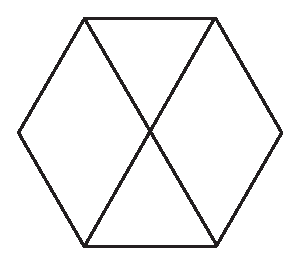
\includegraphics{PS/hex42.eps}
  \caption{A hexagonal cluster with context $(4,2)$.}
  \label{fig:hex42}
\end{figure}

\item\label{app:hex6} If the hexagonal cluster has an upright
diagonal with context $(4,2)$, and if there is one unmasked flat
quarter (Figure~\ref{fig:hex42a}, let $\{F\}$ be the set of four
subregions around the upright diagonal. (That is, take all
subregions except for the flat quarter.) In the following
inequality and Inequality \ref{app:hex7}, let $\sigma_R^+$ be
defined as $\sigma_R$ on quarters, and $\vor_x$ on other anchored
simplices.  $\tau_R^+$ is the adapted squander function.
    $$
    \begin{array}{lll}
    \sum_{(4)}\sigma_R^+ &< -0.253,\\
    \sum_{(4)}\tau_R^+ &> 0.4686.\\
    \end{array}
    %\oldlabel{eqn:4.6.6}
    $$
\begin{figure}[htb]
  \centering
  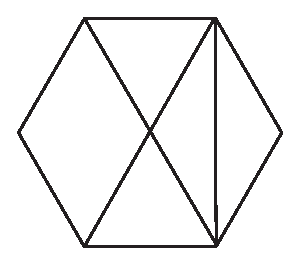
\includegraphics{PS/hex42a.eps}
  \caption{A hexagonal cluster with context $(4,2)$.}
  \label{fig:hex42a}
\end{figure}


\item\label{app:hex7} If the hexagonal cluster has an upright
diagonal with context $(4,2)$, and if there are two unmasked flat
quarters (Figure~\ref{fig:hex42b}), let $\{F\}$ be the set of four
subregions around the upright diagonal. (That is, take all
subregions except for the flat quarters.)
    $$
    \begin{array}{lll}
    \sum_{(4)}\sigma_R^+ &< -0.2,\\
    \sum_{(4)}\tau_R^+ &> 0.3992.\\
    \end{array}
    %\oldlabel{eqn:4.6.7}
    $$
\begin{figure}[htb]
  \centering
  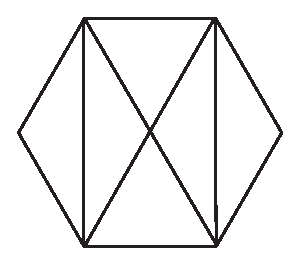
\includegraphics{PS/hex42b.eps}
  \caption{A hexagonal cluster with context $(4,2)$.}
  \label{fig:hex42b}
\end{figure}

\item\label{app:hex8} If the hexagonal cluster has an upright
diagonal in context $(4,1)$, and if there are no flat quarters,
let $\{F\}$ be the set of four subregions around the upright
diagonal. Assume that the edge opposite the upright diagonal on
the anchored simplex has length at least $2\sqrt2$.
 (See Figure~\ref{fig:hex41}.)
    $$
    \begin{array}{lll}
    \vor_{0,R}(D)+\sum_{(3)}\sigma(Q) &< -0.2187\\
    \tau_{0,R}(D)+\sum_{(3)}\tau(Q) &> 0.518.
    \end{array}
    %\oldlabel{eqn:4.6.8}
    $$
\begin{figure}[htb]
  \centering
  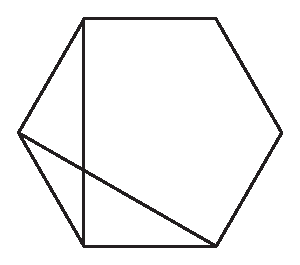
\includegraphics{PS/hex41.eps}
  \caption{A hexagonal cluster with context $(4,1)$.}
  \label{fig:hex41}
\end{figure}

\item\label{app:hex9} In this same context, let $F$ be the
pentagonal subregion along the upright diagonal. It satisfies
    \begin{eqnarray}
    \vor_0 &< -0.137,\\
    \tau_0 &> 0.31.
    \end{eqnarray}
    %\oldlabel{eqn:4.6.9}

\item\label{app:hex10} If the hexagonal cluster has an upright
diagonal in context $(4,1)$, and if there is one unmasked flat
quarter, let $\{F\}$ be the set of four subregions around the
upright diagonal. Assume that the edge opposite the upright
diagonal on the anchored simplex has length at least $2\sqrt2$.
 (There are five subregions, shown in Figure~\ref{fig:hex41a}.)
    $$
    \begin{array}{lll}
    \vor_{0,R}(D)+\sum_{(3)}\sigma(Q) &< -0.1657,\\
    \tau_{0,R}(D)+\sum_{(3)}\tau(Q) &> 0.384.
    \end{array}
    %\oldlabel{eqn:4.6.10}
    $$
\begin{figure}[htb]
  \centering
  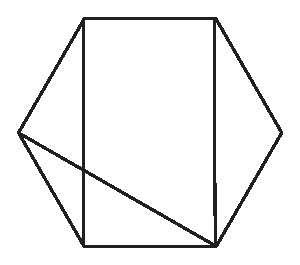
\includegraphics{PS/hex41a.eps}
  \caption{A hexagonal cluster with context $(4,1)$.}
  \label{fig:hex41a}
\end{figure}

\item\label{app:hex11} In this same context, let $F$ be the
quadrilateral subregion in Figure~\ref{fig:hex41a}. It satisfies
    $$
    \begin{array}{lll}
    \vor_0 &< -0.084,\\
    \tau_0 &> 0.176.
    \end{array}
    %\oldlabel{eqn:4.6.11}
    $$


\end{enumerate}


\subsection{Proof of inequalities}
\label{app:hexquad}


\begin{proposition}  Inequalities \ref{app:hex1} --\ref{app:hex11}  are valid.
\end{proposition}

 We prove the inequalities in reverse order \ref{app:hex11}--
\ref{app:hex1}. The bounds\footnote{\calc{148776243}} %2002_IV_A13
   $\vor_0<0.009$ and $\tau_0>0.05925$
%from [$\A_{13}$]
for what a flat quarters with diagonal $\sqrt8$  will be used
repeatedly.  Some of the proofs will make use of tcc-bounds, which
are described in \ref{x-4.10}.
% [Section~5.2]

\begin{proof}
({\it Inequality \ref{app:hex10} and Inequality \ref{app:hex11}.})
Break the quadrilateral cluster into two simplices $S$ and $S'$
along the long edge of the anchored simplex $S$.  The anchored
simplex $S$ satisfies $\tau(S)\ge0$, $\sigma(S)\le0$.  The other
simplex satisfies $\tau_0(S')>0.176$ and $\vor_0(S')<-0.084$ by an
interval calculation.\footnote{\calc{938091791}} % (* kc group 18.16 : app:p11 *)
%\footnote{\calc{}} \ref{app:p11}..
  This gives Inequality \ref{app:hex11}.  For Inequality
\ref{app:hex10}, we combine these bounds with the linear
programming bound on the four anchored simplices around the
upright diagonal.  From a series of
inequalities%
\footnote{\calc{815492935}, \calc{187932932}, \calc{485049042},
\calc{835344007}}
%    [$\A_2$]{part} --
%    [$\A_{7}$]{part},
%    [$\A_{22}$]{part},
%    [$\A_{24}$]{part},
we find that they score $<-0.0817$ and squander $>0.208$.  Adding
these to the bounds from Inequality \ref{app:hex11}, we obtain
Inequality \ref{app:hex10}.
\end{proof}

\begin{proof}
{\it (Inequality (\ref{app:hex8}) and (\ref{app:hex9}).)} The
pentagon is a union of an anchored simplex and a quadrilateral
region. LP-bounds similar to those in the previous paragraph and
based on the inequalities of Section~\ref{sec:loops} show that the
loop scores at most $-0.0817$ and squanders at least $0.208$.  If we
show that the quadrilateral satisfies
    \begin{eqnarray}
    \vor_0&<-0.137,\label{eqn:hexquadsig}\\
    \tau_0&>0.31,\label{eqn:hexquadtau}
    \end{eqnarray}
then Inequalities (\ref{app:hex8}) and (\ref{app:hex9}) follow. If
by deformations a diagonal of the quadrilateral drops to
$2\sqrt2$, then the result follows
 %from Inequalities \ref{app:p8} and
interval calculations.\footnote{\calc{148776243},\calc{468742136}} % (* kc group 18.15 : app:p8 *)
 %[$\A_{13}$]{part-4}.
 By this we may now assume that the
quadrilateral has the form
    $$(a_1,2,a_2,2,a_3,2,a_4,b_4),\quad a_2,a_3\in\{2,2t_0\}.$$
If the diagonals drop under $3.2$ and $\max(a_2,a_3)=2t_0$, again
the result follows from
 %Inequalities \ref{app:p8} and
 interval
calculations.\footnote{calc{148776243},\calc{468742136}} % (* kc group 18.15 : app:p8 *)
%[$\A_{13}$]{part-4}.
If the diagonals drop under $3.2$ and $a_2=a_3=2$, then the result
follows from further interval
calculations.\footnote{\calc{128523606}} %[$\A_{19}$]{part-4}.
So finally we attain by deformations $b_4=2\sqrt2$ with both
diagonals greater than $3.2$. But this does not exist, because
    $$\Delta(4,4,4,3.2^2,4,8,3.2^2)<0.$$
\end{proof}


\begin{proof}
{\it (Inequality \ref{app:hex5}, Inequality \ref{app:hex6}, and
Inequality \ref{app:hex7}.)} Inequalities \ref{app:hex7} are
derived in Section~\ref{x-5.11}. Inequalities \ref{app:hex5},
\ref{app:hex6} are LP-bounds based on interval
calculations.\footnote{\calc{815492935}, \calc{187932932},
\calc{485049042}}
% [$\A_2$]{part-4}, [$\A_7$]{part-4}, [$\A_{22}$]{part-4}.
\end{proof}

\begin{proof} {\it (Inequality \ref{app:hex4}.)} Deform as in
Section~\ref{sec:BER}. If at any point a diagonal of the
quadrilateral drops to $2\sqrt2$, then the result follows from
interval
calculations\footnote{\calc{148776243}} % IVA13_ [$\A_{13}$]{part-4}
and Inequality \ref{app:hex11}:
    $$
    \begin{array}{lll}
    \vor_0 &< 0.009 -0.084 = -0.075,\\
    \tau_0 &> 0 + 0.176 = 0.176,\\
    \end{array}
    $$
Continue deformations until the quadrilateral has the form
    $$(a_1,2,a_2,2,a_3,2,a_4,b_4),\quad a_2,a_3\in\{2,2t_0\}.$$
There is necessarily a diagonal of length $\le3.2$, because
    $$\Delta(4,4,3.2^2,8,4,3.2^2)<0.$$
Suppose the diagonal between vertices $v_2$ and $v_4$ has length
at most $3.2$.  If $a_2=2t_0$ or $a_3=2t_0$, the result follows
from interval calculations\footnote{\calc{148776243}} % IVA13_ [$\A_{13}$]{part-4}
and Inequality \ref{app:hex11}. Take $a_2=a_3=2$. Inequality
\ref{app:hex4} now follows from interval
calculations.\footnote{\calc{128523606}} % IVA19_ [$\A_{19}$]{part-4}.
\end{proof}

\begin{proof}
{\it (Inequality \ref{app:hex3}).}
 We prove that the quadrilateral
satisfies
    $$
    \begin{array}{lll}
    \vor_0 &< -0.168\\
    \tau_0 &> 0.352.\\
    \end{array}
    $$
There are two types of quadrilaterals.  In (a), there are two flat
quarters whose central vertices are opposite corners of the
hexagon.  In (b), the flat quarters share a vertex.
  We consider case (a) first.

Case (a). We deform the quadrilateral as in
Section~\ref{sec:BER}.%{part-4}.
If at any point there is a
diagonal of length at most $3.2$, the result follows from
Inequality \ref{app:hex10} and Inequality \ref{app:hex11}.
Otherwise, the deformations give us a quadrilateral
    $$(a_1,2,a_2,2t_0,a_3,2,a_4,2), \quad a_i \in\{2,2t_0\}.$$
The tcc approximation now gives the result (see
\Chap~\ref{x-4.11}).
%[5.3)]{part-4}.

Case (b). Label the vertices of the quadrilateral
 $v_1,\ldots,v_4$, where $(v_1,v_2)$ and $(v_1,v_4)$
are the diagonals of the flat quarter.  Again, we deform the
quadrilateral.  If at any point of the deformation, we find that
$|v_1-v_3|\le 3.2$, the result follows from Inequalities
\ref{app:hex10}, \ref{app:hex11}. If during the deformation
$|v_2-v_4|\le2\sqrt2$, the result follows from
%[$\A_{13}$]{part-4}
interval calculations.\footnote{\calc{148776243},\calc{315678695}} % (* kc group 18.14 : app:p3  *)
 % IVA13_
 % \ref{app:p3}.
If the diagonal $(v_2,v_4)$ has length at least
$3.2$ throughout the deformation, we eventually obtain a
quadrilateral of the form
    $$(a_1,2t_0,a_2,2,a_3,2,a_4,2t_0),\quad a_i\in\{2,2t_0\}.$$
But this does not exist:
$$\Delta(4,4,3.2^2,(2t_0)^2,(2t_0)^2,3.2^2)<0.$$

We may assume that $|v_2-v_4|\in[2\sqrt2,3.2]$.  The result now
follows from interval calculations.\footnote{\calc{315678695}} % (* kc group 18.14 : app:p3  *)  \ref{app:p3}.
\end{proof}

\begin{proof}
{\it (Inequality \ref{app:hex2}).} This case requires more effort.
We show that
    $$
    \begin{array}{lll}
    \vor_0 &< -0.221\\
    \tau_0 &> 0.486\\
    \end{array}
    $$
Label the corners $(v_1,\ldots,v_5)$ cyclically with $(v_1,v_5)$ the
diagonal of the flat quarter in the hexagonal cluster. We use the
deformation theory of \Chap~\ref{sec:BER}.
%{part-4}.
The proof appears in
steps $(1),\ldots,(6)$.

(1) If during the deformations, $|v_1-v_4|\le3.2$ or
$|v_2-v_5|\le3.2$, the result follows from Inequalities
\ref{app:hexquad} and \ref{app:hex11}.  We may assume this does
not occur.

(2) If an edge $(v_1,v_3)$, $(v_2,v_4)$, or $(v_3,v_5)$ drops to
$2\sqrt2$, continue with deformations that do not further decrease
this diagonal. If $|v_1-v_3|=|v_3-v_5|=2\sqrt2$, then the result
follows from
    %[$\A_{13}$]{part-4}
interval calculations.\footnote{\calc{148776243},\calc{673399623}} % (* kc group 18.7 : app:p2a  *) % IVA13_
%\ref{app:p2a}.

If we have $|v_1-v_3|=2\sqrt2$, deform the figure to the form
    $$(a_1,2,a_2,2,a_3,2,a_4,2,a_5,2t_0),\quad a_2,a_4,a_5\in\{2,2t_0\}.$$
Once it is in this form, break the flat quarter $(0,v_1,v_2,v_3)$
from the cluster and deform $v_3$ until $a_3\in\{2,2t_0\}$.  The
result follows from an interval calculation.\footnote{\calc{297256991}} % (* kc group 18.8 : app:p2b *) \ref{app:p2b}.

We handle a boundary case of the preceding calculation separately.
After breaking the flat quarter off, we have the cluster
    $$(a_1,2\sqrt2,a_3,2,a_4,2,a_5,2t_0),\quad a_3,a_4,a_5\in\{2,2t_0\}.$$
If $|v_1-v_4|=3.2$, we break the quadrilateral cluster into two
pieces along this diagonal and use interval calculations\footnote{\calc{861511432}} % (* kc group 18.9 : app:p2c *)
%\ref{app:p2c}
to conclude the result. This completes the analysis
of the case $|v_1-v_3|=2\sqrt2$.

(3) If $|v_2-v_4|\le3.2$, then deform until the cluster has the
form
    $$(a_1,2,a_2,2,a_3,2,a_4,2,a_5,2t_0),\quad a_1,a_3,a_5\in\{2,2t_0\}.$$
Then cut along the special simplex to produce a quadrilateral.
Disregarding cases already treated by the interval calculations,\footnote{\calc{861511432}} % (* kc group 18.9 : app:p2c *)
%\ref{app:p2c},
we can deform it to
    $$(a_1,2,a_2,2\sqrt2,a_4,2,a_5,2t_0),\quad a_i\in\{2,2t_0\},$$
with diagonals at least $3.2$. The result now follows from
interval calculations.\footnote{\calc{746445726}} % (* kc group 18.10 : app:p2d *) \ref{app:p2d}.

In summary of (1), (2), (3), we find that by disregarding cases
already considered, we may deform the cluster into the form
    $$(a_1,2,a_2,2,a_3,2,a_4,2,a_5,2t_0),\quad a_i\in\{2,2t_0\},$$
$|v_1-v_3|>2\sqrt2$, $|v_3-v_5|>2\sqrt2$, $|v_2-v_4|>3.2.$

(4) Assume $|v_1-v_3|,|v_3-v_5|\le3.2$. If
$\max(a_1,a_3,a_5)=2t_0$, we invoke
 interval calculations\footnote{\calc{148776243},\calc{297256991}} % (* kc group 18.8 : app:p2b *) % IVA13_
%\ref{app:p2b}
%and [$\A_{13}$]{part-4}
to prove the
inequalities.
 So we may assume $a_1=a_3=a_5=2$.  The result now follows from
interval calculations.\footnote{\calc{897046482}} % (* kc group 18.11 : app:p2e *) \ref{app:p2e}.
This completes the case
$|v_1-v_3|,|v_3-v_5|\le3.2$.

(5) Assume $|v_1-v_3|,|v_3-v_5|\ge3.2$. We deform to
    $$(a_1,2,a_2,2,a_3,2,a_4,2,a_5,2t_0),\quad a_i\in\{2,2t_0\}.$$
If $a_2=2t_0$ and  $a_1=a_3=2$, then the simplex does not exist by
Section~\ref{x-5.6}.  %[5.6]{part-4}.
Similarly, $a_4=2t_0$, $a_5=a_3=2$ does not exist. The tcc bound
gives the result except when $a_2=a_4=2$. The condition
$|v_2-v_4|\ge3.2$ forces $a_3=2$. These remaining cases are
treated with interval calculations.\footnote{\calc{928952883}} % (* kc group 18.12 : app:p2f *) \ref{app:p2f}.

(6) Assume $|v_1-v_3|\le3.2$ and $|v_3-v_5|\ge3.2$. This case
follows from deformations, interval
calculations.\footnote{\calc{297256991},\calc{673800906}} % (* kc group 18.13 : app:p2g *) % (* kc group 18.8 : app:p2b *) \ref{app:p2b},
%and \ref{app:p2g}.
This completes the proof of Inequalities
\ref{app:hex2}.
\end{proof}

\smallskip
\begin{proof}
{\it (Inequality \ref{app:hex1}).} Label the corners of the hexagon
$v_1,\ldots,v_6$.  The proof to this inequality is similar to the
other cases.  We deform the cluster by the method of
\Chap~\ref{sec:BER} until it breaks into pieces that are small
enough to be estimated by interval calculations. If a diagonal
between opposite corners has length at most $3.2$, then the hexagon
breaks into two quadrilaterals and the result follows from
Inequality \ref{app:hexquad}.

If a flat quarter is formed during the course of deformation, then
the result follows from Inequality \ref{app:hex2} and interval
calculations.\footnote{\calc{148776243}} % IVA13_ [$\A_{13}$]{part-4}.
Deform until the hexagon
has the form
    $$(a_1,2,a_2,2,\ldots,a_6,2),\quad a_i\in\{2,2t_0\}.$$
We may also assume that the hexagon is convex (see
\Chap~\ref{x-4.13}). % [Section~4.11]{part-4}).

If there are no special simplices, we consider the tcc-bound. The
tcc-bound implies Inequality \ref {app:hex1}, except when $a_i=2$,
for all $i$. But if this occurs, the perimeter of the convex
spherical polygon is $6\arc(2,2,2)=2\pi$.  Thus, there is a pair
of antipodal points on the hexagon.  The hexagon degenerates to a
lune with vertices at the antipodal points.  This means that some
of the angles of the hexagon are $\pi$.   One of the tccs has the
form $C(2,1.6,\pi)$, in the notation of \Chap~\ref{x-4.11}.
%[Lemma~4.11]{part-4}.
With this extra bit of information, the
tcc bound implies Inequality \ref {app:hex1}.

If there is one special simplex, say $|v_5-v_1|\in[2\sqrt2,3.2]$,
we remove it. The score of the special simplex is\footnote{\calc{148776243}} % IVA13_
%[Inequalities $\A_{13}$]{part-4}
    $$
    \begin{array}{lll}
    \vor_0 &< 0,\quad \tau_0>0.05925,\quad\text{if }\max(|v_1|,|v_5|)=2t_0,\\
    \vor_0 &< 0.0461,\quad \tau_0>0,\quad\text{if }|v_1|=|v_5|=2,\\
    \end{array}
    $$
The resulting pentagon can be deformed. If by deformations, we
obtain $|v_2-v_5|=3.2$ or $|v_1-v_4|=3.2$, the result follows from
Inequalities \ref{app:hexquad} and two interval calculations.%
\footnote{\calc{725257062}, \calc{977272202}}

%\oldlabel{A.4.6.1.a}

%$\vor_0 < -0.212 -0.0461 +0.137$, if $y_4=3.2$,
%$y_5\in[2\sqrt2,3.2]$. \refno{725257062\dag}

%$\tau_0 > 0.54525 - 0 - 0.31$. if $y_4=3.2$,
%$y_5\in[2\sqrt2,3.2]$. \refno{977272202\dag}

If $|v_5-v_1|=2\sqrt2$, we use Inequality \ref{app:hex2} and
interval calculations\footnote{\calc{148776243}} % IVA13_ [$\A_{13}$]{part-4}
unless $|v_1|=|v_5|=2$. If $|v_1|=|v_5|=2$, we use  interval
calculations.\footnote{\calc{377409251}} % (* 18.3 : app:p1b *) \ref{app:p1b}.
If a second special simplex forms during the deformations, the
result follows from interval calculations.\footnote{\calc{586214007}} % (* 18.4 : app:p1c *) \ref{app:p1c}.

The final case of Inequality \ref{app:hex1}  to consider is that
of two special simplices. We divide this into two cases. (a) The
central vertices of the specials are $v_2$ and $v_6$.  (b) The
central vertices are opposite $v_1$ and $v_4$. In case (a), the
result follows by deformations and interval calculations.\footnote{\calc{89384104}} % (* 18.5 : app:p1d *)
%\ref{app:p1d}.
In case (b), the result follows by deformations and interval
calculations.\footnote{\calc{859726639}} % (* kc group 18.6 : app:p1e  *) \ref{app:p1e}.
This completes the proof of
Inequalities \ref{app:hex1} and the proof of the Proposition.
\end{proof}
